\subsection{Permutation Argument}

\emph{Step 1: Label and define permutation index polynomial $S$}

Permutation Argument explicitly specifies the exact location of the equal value, just as $V_3(1) = V_5(0)$ shown in Figure \ref{fig:permutation-index-polynomial}. Therefore, we need to define a new polynomial to represent the index correspondence between different polynomials.

\begin{figure}[!ht]
    \centering
    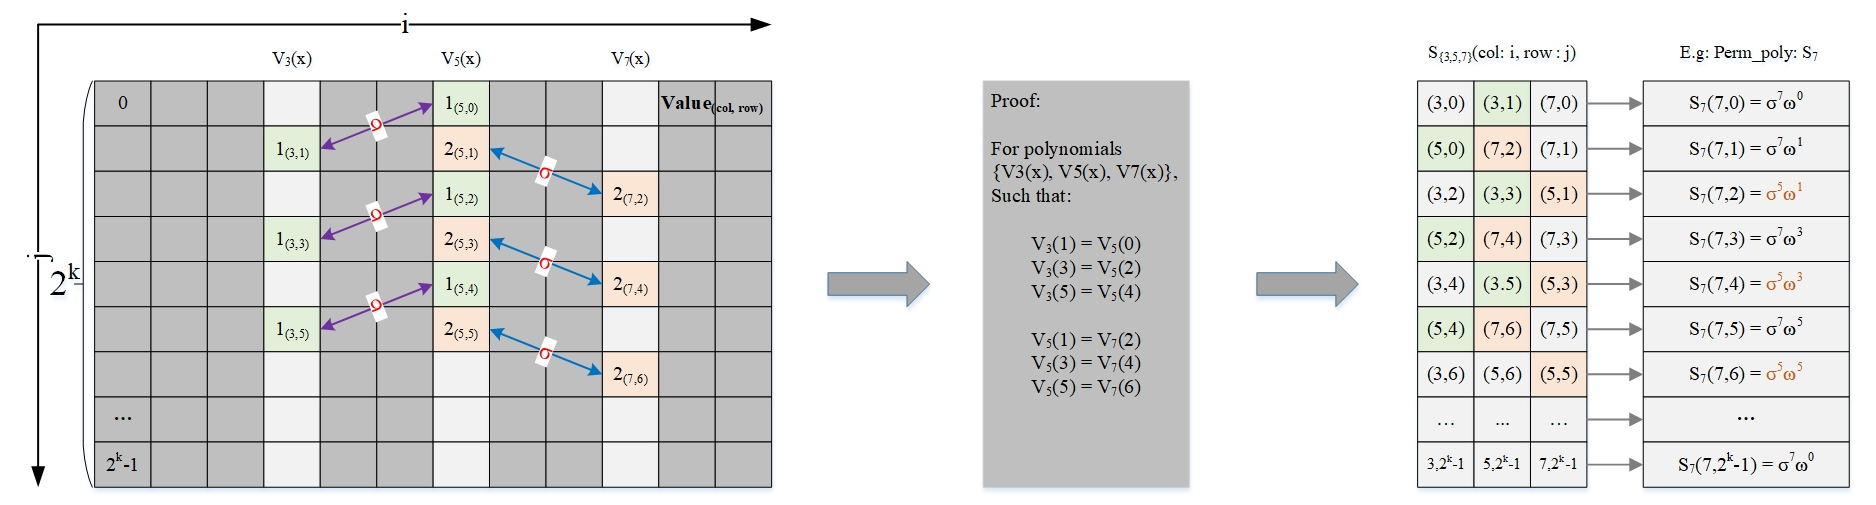
\includegraphics[width=\textwidth]{permutation-index-polynomial.jpg}
    \caption{Permutation index polynomial}
    \label{fig:permutation-index-polynomial}
\end{figure}

Since different polynomials correspond to different column indices, we can distinguish different evaluation domains by introducing column indices (distinguished through introducing a domain of size $n$ in Plonk, i.e.\ if there are $k$ polynomials, the domain size of \verb|perm_index_poly| is $kn$). The mapping can be expressed as
\[ S(\text{col:}i, \text{row:}j)=\sigma^{i'} \omega^{j'}. \]

Taking the polynomial $V_7(X)$ of column index = 7 as an example, the truth value of its corresponding permutation index polynomial $S_7(\text{col:}i, \text{row:}j)$ is shown in the right side of Figure \ref{fig:permutation-index-polynomial}.

\emph{Step 2: Generate the proof}

For the permutation index polynomial set $S = \{S_i\}$ generated based on step 1, we need to ensure the following equation holds:
\[
    \prod_{j=0}^{n-1} \frac{\left(V_3(\omega^j)+\beta \cdot \sigma^3 \cdot \omega^j+\gamma\right) \left(V_5(\omega^j)+\beta \cdot \sigma^5 \cdot \omega^j+\gamma\right) \left(V_7(\omega^j)+\beta \cdot \sigma^7 \cdot \omega^j+\gamma\right)} {\left(V_3(\omega^j)+\beta \cdot S(3, \omega^j)+\gamma\right) \left(V_5(\omega^j)+\beta \cdot S(5,\omega^{j})+\gamma\right) \left(V_7(\omega^j)+\beta \cdot S(7,\omega^{j})+\gamma\right)} = 1.
\]

\emph{Note:} If we reorder the indices of three polynomials (starting from 0 regardless of the original order, then the polynomial indices will be 0, 1 and 2 successively), the above equation can be simply expressed as
\[ \prod_{i=0}^{m-1} \prod_{j=0}^{n-1} \frac{V_i(\omega^j)+\beta \cdot \sigma^i \cdot \omega^j+\gamma}{V_i(\omega^j)+\beta \cdot S_i(\omega^j)+\gamma}=1. \]

where the permutation index polynomial is defined as
\[ S_{\text{col:}i}\left(\omega^{\text{row:}j}\right)=\sigma^{i'} \omega^{j'}. \]

The principle is shown in Figure \ref{fig:accumulator-polynomial}.

\begin{figure}[!ht]
    \centering
    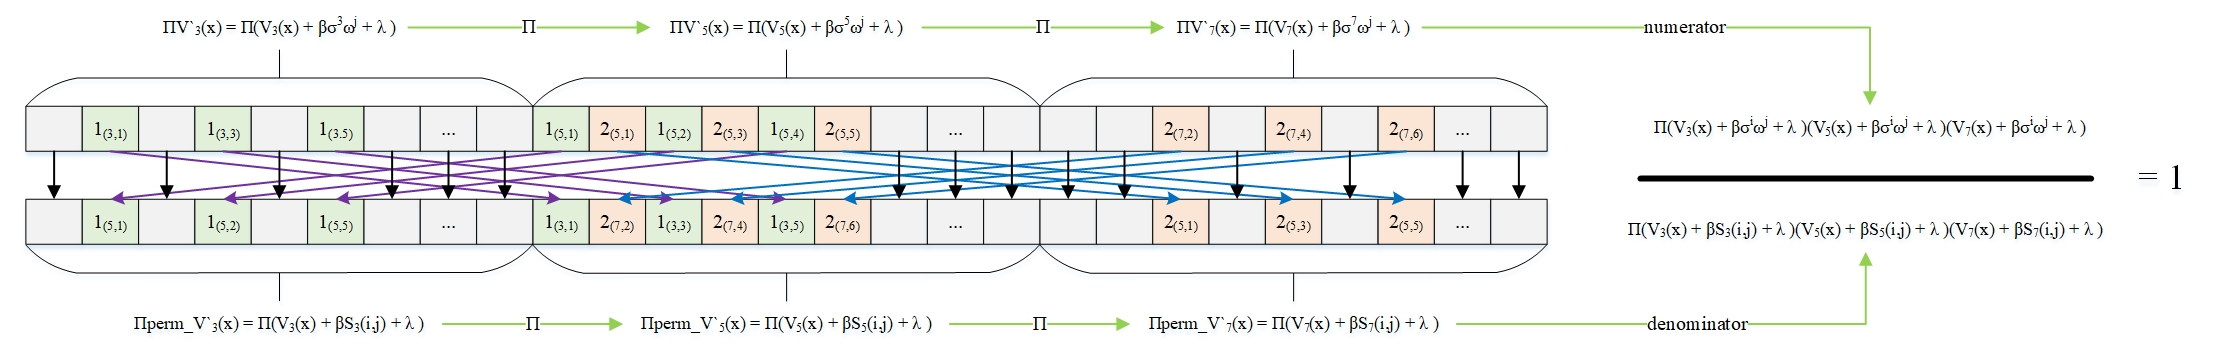
\includegraphics[width=\textwidth]{accumulator-polynomial.jpg}
    \caption{Accumulator polynomial}
    \label{fig:accumulator-polynomial}
\end{figure}

Due to the introduction of random numbers $\beta$ and $\gamma$, we can guarantee the two cells connected by purple lines and blue lines in Figure \ref{fig:accumulator-polynomial} to be equal with a probability close to 1 if and only if the copy constraints are satisfied according to Schwartz-Zippel Lemma. Finally, the multiplication result of the numerators is equal to that of denominators. Define the multiplicative polynomial $Z_P$ as follows:
\begin{align*}
    Z_P(W^0) &= 1, \\
    Z_P(W^{j+1}) &= \prod_{h=0}^j \prod_{i=0}^{m-1}\frac{V_i(\omega^h)+\beta \cdot \sigma^i \cdot \omega^h+\gamma}{V_i(\omega^h)+\beta \cdot S_i(\omega^h)+\gamma} \\
    &= Z_P(W^j)\prod_{i=0}^{m-1}\frac{V_i(\omega^{j})+\beta \cdot \sigma^{i} \cdot \omega^j+\gamma}{V_i(\omega^j)+\beta \cdot S_i(\omega^j)+\gamma}.
\end{align*}

It should satisfy the following constraints
\begin{align*}
    Z_P(\omega X) \prod_{i=0}^{m-1}\left(V_i(x)+\beta \cdot S_i(X)+\gamma\right) - Z_P(X) \prod_{i=0}^{m-1}\left(V_i(X)+\beta \cdot \sigma^{i} \cdot X+\gamma\right)=0, \\
    l_0 \cdot\left(1-Z_P(X)\right)=0.
\end{align*}

For further understanding of the principle, see Permutation Argument \cite{website:permutation-argument}.
